\let\negmedspace\undefined
\let\negthickspace\undefined
\documentclass[journal]{IEEEtran}
\usepackage[a5paper, margin=10mm, onecolumn]{geometry}
%\usepackage{lmodern} % Uncomment if needed for pdflatex
\usepackage{tfrupee} % Include tfrupee package

\setlength{\headheight}{1cm} % Set the height of the header box
\setlength{\headsep}{0mm}     % Set the distance between the header box and the top of the text

\usepackage{gvv-book}
\usepackage{gvv}
\usepackage{cite}
\usepackage{amsmath,amssymb,amsfonts,amsthm}
\usepackage{algorithmic}
\usepackage{graphicx}
\usepackage{textcomp}
\usepackage{xcolor}
\usepackage{txfonts}
\usepackage{listings}
\usepackage{enumitem}
\usepackage{mathtools}
\usepackage{gensymb}
\usepackage{comment}
\usepackage[breaklinks=true]{hyperref}
\usepackage{tkz-euclide} 
\usepackage{listings}
%\usepackage{gvv}                                        
\def\inputGnumericTable{}                                 
\usepackage[latin1]{inputenc}                                
\usepackage{color}                                            
\usepackage{array}                                            
\usepackage{longtable}                                       
\usepackage{calc}                                             
\usepackage{multirow}                                         
\usepackage{hhline}                                           
\usepackage{ifthen}                                           
\usepackage{lscape}
\usepackage{tikz}
\usepackage{circuitikz}
\usepackage{standalone} % For including external TikZ files

\begin{document}

\bibliographystyle{IEEEtran}
\vspace{3cm}

\title{9.5.14}
\author{EE24BTECH11066 - YERRA AKHILESH}
% \maketitle
% \newpage
% \bigskip
{\let\newpage\relax\maketitle}

\renewcommand{\thefigure}{\theenumi}
\renewcommand{\thetable}{\theenumi}
\setlength{\intextsep}{10pt} % Space between text and floats

\numberwithin{equation}{enumi}
\numberwithin{figure}{enumi}
\renewcommand{\thetable}{\theenumi}
\textbf{Question}:\\
For the following differential equation, find the particular solution satisfying the given condition:\\

$\frac{dy}{dx} - \frac{y}{x} + \csc \brak{\frac{y}{x}} = 0; y=0$ when $x=1$\\

\textbf{Solution: }
Given  Differential equation:   
\begin{align}
    \frac{dy}{dx} - \frac{y}{x} + \csc \brak{\frac{y}{x}}=0
\end{align}
let $t$ be a variable,
\begin{align}
    \frac{y}{x} = t\\
    y=xt
\end{align}
Differentiate on both sides with $x$,
\begin{align}
    \frac{dy}{dx} = t + x\frac{dt}{dx}
\end{align}
Substitute the above $\frac{dy}{dx}$ in given differential equation,
\begin{align}
    t+x\frac{dt}{dx}-t+\csc(t)=0\\
    \frac{dt}{dx}= -\frac{\csc(t)}{x}\\
    -\sin t \, dt = \frac{dx}{x}
\end{align}
Integrating on both sides, 
\begin{align}
    \int -\sin t \, dt = \int \frac{1}{x} \, dx\\
    \cos t = \log \abs{cx}
\end{align}
where $c$ be integrating constant and it can be obtained by substituting intial values$\brak{y=0, x=1}$\\

On substituting, 
\begin{align}
    c = e
\end{align}
Therefore final solution for $y(x)$ by substituting $t=\frac{y}{x}$, 
\begin{align}
    \cos \frac{y}{x} = (1 + \log x)\\  
    y(x) = x \cdot \cos^{-1}(1+\log x)
\end{align}
Now let us verify this computationally
From definition of $\frac{dy}{dx}$,
\begin{align}
    y_{n+1}=y_{n}+\frac{dy}{dx}\cdot h
    \label{0.15}
\end{align}
(where h is small number tending to zero)
From the differential equation given,
\begin{align}
    \frac{dy}{dx}=\frac{y}{x} - \csc \frac{y}{x}
    \label{0.16}
\end{align}
By substituting \ref{0.16} in \ref{0.15},
\begin{align}
    y_{n+1}=y_{n}+\brak{\frac{y_n}{x_n} - \csc \frac{y_n}{x_n}}\cdot h
\end{align}
By taking $x_1=0.2 \text{ and } y_1=0.4361$  and $h=0.0032$ going till $x=1$ by iterating through the loop and finding $y_2,y_3,\cdots , y_{500}$ and plotting the graph, we can verify if the function we got by solving the differential equation mathematically.\\
\begin{figure}[H]
    \centering
    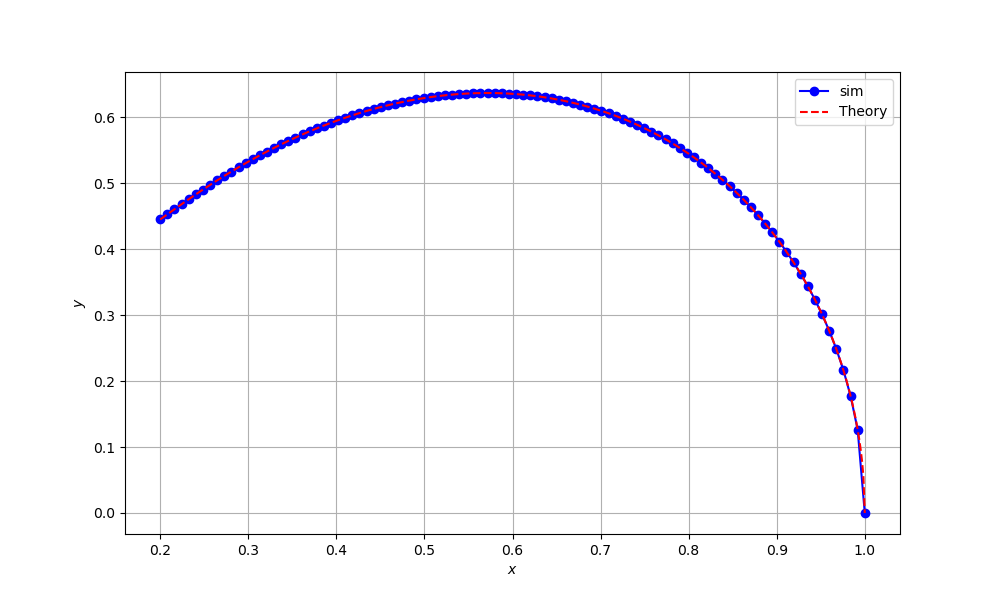
\includegraphics[width = \columnwidth]{figs/Figure_1.png}
\end{figure}


\end{document}
